
\documentclass{article}
\usepackage{graphicx}
\usepackage[top=3cm]{geometry}
\usepackage{tabularray}
\usepackage{afterpage}
\usepackage{amsmath,amssymb}
\usepackage{listings}
\usepackage{subcaption}
\usepackage{mwe}
\usepackage{epstopdf}
\usepackage{textgreek}

\lstset{language=Matlab}
\graphicspath{{./}}
\author{ Harshal Varpe}
\title{ECE 8540 Analysis of Tracking System\\
\Large Lab 7 Report: Viterbi Algorithm }

\begin{document}
\maketitle

\section{Introduction}\label{sec:intro}

This lab dealt with Hidden Markov Model with two possible states: H (High GC content) and L(Low GC content). From each state (H and L), we have different probabilities for different nucleotides (A, G, C, T) in DNA to occur. The students were to implement a Viterbi algorithm to find the most probable path to create a certain sequence of a protein/DNA. The Viterbi algorithm is a dynamical programming algorithm that helps us compute the most probable path. \\
For this lab, the students had to find out the most probable path to achieve two different DNA sequences. The two DNA sequences are: "GGCACTGAA", "TCAGCGGCT" \\
\begin{figure}[!htb]
\begin{center}
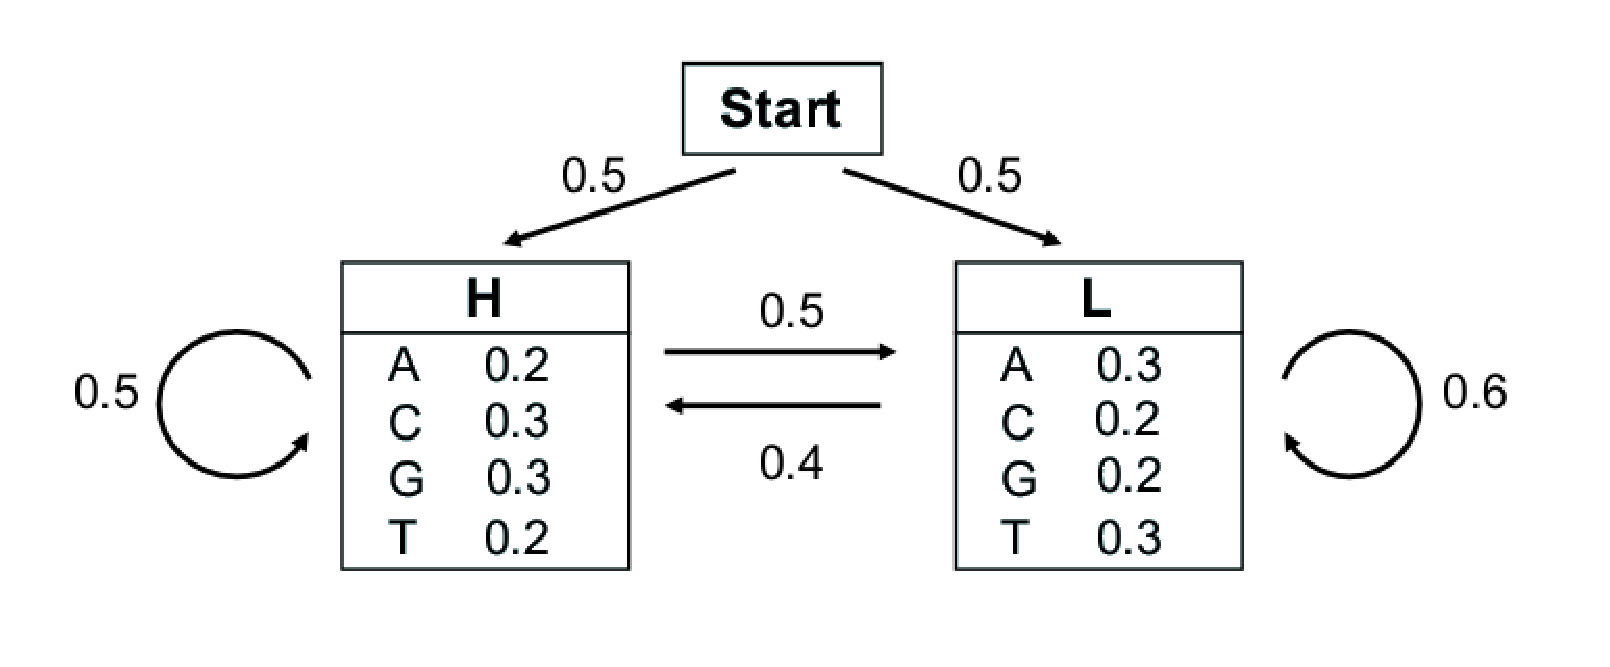
\includegraphics[scale=0.5]{HMM.eps}
\caption{Hidden Markov Model}
\label{Fig:1}
\end{center}
\end{figure}

\section{Methods and Implementation}\label{sec:methImp}
\subsection{Method}\label{sec:Meth}
The two states for the given Hidden Markov Model(HMM) are H, and L. Figure \ref{Fig:1} shows the Hidden Markov Model used for the given problem. The prior probabilities are 0.5 and 0.5. The state transition probabilities are \{0.5,0.5\} for H and \{0.4,0.6\} for L. For the state H, the emission probabilities of four different values/nucleotides (A, C, G, T) are \{ 0.2,0.3,0.3,0.2\}. Similarly, the emission probabilities for the four nucleotides for state L are \{ 0.3,0.2,0.2,0.3\}.\\

Once all the probabilities are known, the Viterbi calculations can be performed. It is important to note that for the calculations, we use sums of the $log_2$ of the probabilities. The Viterbi equation is given below.\\

The probability of the most probable path ending in state $l$ with observation $i$ is :
\begin{equation}
	p_l(i,x) = e_l(i) \cdot \displaystyle\max_k(p_k(j,x-1) \cdot p_{kl})
\end{equation}
Where $e_l(i)$ is the probability to observe element $i$ in state $l$, $p_k(j,x-1)$ is the probability of the most probable path ending at position $x-1$ in state $k$ with element $j$, and the last term $p_{kl}$ is the probability of the transition from state $l$ to state $k$.\\

For example, for the sequence 'GGCACTGAA', the probability of the mosr probable path ending in state $H$ with observation "A" at the 4th position is given by equation:
\begin{equation}
	p_H(A,4) = e_H(A) \cdot max(p_L(C,3) \cdot p_{LH}, p_H(C,3) \cdot p_{HH} )
\end{equation}

\subsection{Implementation}\label{sec:Imp}
In this subsection, I will briefly go over the implementation steps of the Viterbi Algorithm.
\begin{enumerate}
\item Calculation of the probability that the first nucleotide is emitted by states H and L.
\item Calculation of the probability that the remaining nucleotides are emitted by states H and L.
\item backtracking
In this step, we backtrack all the probabilities of finding the most probable path. We compare the probabilities that a nucleotide came from state H or L. The higher probability is chosen.
\end{enumerate}

\section{Result}\label{sec:res}
In the table \ref{Tab:1}, we can see the probabilities of each of the nucleotides from states H and L for sequence "GGCACTGAA." Based on the numbers, we can see that the most probable path is: \textbf {HHHLLLLLL}.
The boldfaced numbers in the table denote the highest probability.\\



\begin{table}[]
\begin{center}
\begin{tabular}{|c|c|c|}
\hline
Nucleotide & H Probabilities & L  Probabilities   \\ \hline
G & \textbf{-2.73} & -3.32 \\ \hline
G & \textbf{-5.471} & -6.05 \\ \hline
C & \textbf{-8.21} & -8.79 \\ \hline
A & -11.53  & \textbf{-10.94} \\ \hline
C & -14.00 & \textbf{-14.00} \\ \hline
T & -17.32 & \textbf{-16.488} \\ \hline
G & -19.53 & \textbf{-19.53} \\ \hline
A & -22.86 & \textbf{-22.01}\\ \hline
A & -25.65 & \textbf{-24.48} \\ \hline
\end{tabular}
\end{center}
\caption{Table of Probabilities for Sequence 'GGCACTGAA'}
\label{Tab:1}
\end{table}

Similarly, in table \ref{Tab:2}, we can see the probabilities of each of the nucleotides from states H and L for sequence "TCAGCGGCT." Based on the numbers, we can see that the most probable path is: \textbf {LLLLHHHHL}.\\

\begin{table}[]
\begin{center}
\begin{tabular}{|c|c|c|}
\hline
Nucleotide & H Probabilities   & L Probabilities   \\ \hline
T          & -3.32 & \textbf{-2.73} \\ \hline
C          & -5.79 & \textbf{-5.79} \\ \hline
A          & -9.11 & \textbf{-8.26} \\ \hline
G          & -11.32 & \textbf{-11.32} \\ \hline
C          & \textbf{-14.06}  & -14.38 \\ \hline
G          & \textbf{-16.80} & -17.38 \\ \hline
G          & \textbf{-19.53} & -20.12 \\ \hline
C          & \textbf{-22.27} & -22.86 \\ \hline
T          & -25.59 & \textbf{-25.01} \\ \hline
\end{tabular}
\end{center}
\caption{Table of Probabilities for Sequence 'TCAGCGGCT'}
\label{Tab:2}
\end{table}

\section{Conclusion}\label{sec:conc}
The Viterbi algorithm is a dynamical programming algorithm that is used to compute the most probable path as well as its probability. The algorithm requires knowledge of the parameters of the HMM model and a particular output sequence. The algorithm then finds the state sequence most likely to have generated that output sequence. The Viterbi algorithm provides a computationally efficient method of decoding the DNA sequence. The algorithm is much better than the previous brute force techniques that were computationally expensive.\\

In this Lab, we derived the most probable path for two DNA sequences. The results obtained by the algorithm and those calculated manually were cross-referenced to ensure the algorithm's reliability.



\section{Apendix}\label{sec:apdx}
\begin{lstlisting}[frame=single]
%Lab 7 Viterbi Algorithm
%Harshal Varpe

clear all
clc


in_1 = ['G', 'G', 'C', 'A', 'C', 'T', 'G', 'A', 'A' ];
in_2 = ['T', 'C', 'A', 'G', 'C', 'G', 'G', 'C', 'T' ];
in_seq = {in_1 , in_2};

%define all the probabilities
p_init = log2([0.5,0.5]); % start to state H and L
p_th = log2([0.5,0.5]);% H to H and H to L
p_tl = log2([0.6,0.4]);% L to L and L to H
p_h = log2([0.2,0.3,0.3,0.2]); % ACGT for H
p_l = log2([0.3,0.2,0.2,0.3]); % ACGT for L
p = zeros(length(in_1),2);
% out = zeros(length(in_1),1);
Section
for i = 1:1:length(in_seq)
   a =  in_seq{i};
%    fprintf("%d",length(a));
    for j=1:1:length(a)
%         fprintf("%c\t\t",a(j));
        if(j == 1)
            if(strcmpi(a(j),'A'))
                p(j,1) = p_init(1) + p_h(1);
                p(j,2) = p_init(2) + p_l(1);
                
            elseif(strcmpi(a(j),'C'))
                p(j,1) = p_init(1) + p_h(2);
                p(j,2) = p_init(2) + p_l(2);
                
            elseif(strcmpi(a(j),'G'))
                p(j,1) = p_init(1) + p_h(3);
                p(j,2) = p_init(2) + p_l(3);
                
            else %T
                p(j,1) = p_init(1) + p_h(4);
                p(j,2) = p_init(2) + p_l(4);
                
            end
        else
            if(strcmpi(a(j),'A'))
                p(j,1) = p_h(1) + max([ (p(j-1,1)+p_th(1)),(p(j-1,2)+p_tl(2)) ]);
                p(j,2) = p_l(1) + max([ (p(j-1,1)+p_th(2)),(p(j-1,2)+p_tl(1))]);
                
            elseif(strcmpi(a(j),'C'))
                p(j,1) = p_h(2) + max([ (p(j-1,1)+p_th(1)),(p(j-1,2)+p_tl(2)) ]);
                p(j,2) = p_l(2) + max([ (p(j-1,1)+p_th(2)),(p(j-1,2)+p_tl(1)) ]);
                
            elseif(strcmpi(a(j),'G'))
                p(j,1) = p_h(3) + max([ (p(j-1,1)+p_th(1)),(p(j-1,2)+p_tl(2)) ]);
                p(j,2) = p_l(3) + max([ (p(j-1,1)+p_th(2)),(p(j-1,2)+p_tl(1)) ]);
                
            else %T
                p(j,1) = p_h(4) + max([ (p(j-1,1)+p_th(1)),(p(j-1,2)+p_tl(2)) ]);
                p(j,2) = p_l(4) + max([ (p(j-1,1)+p_th(2)),(p(j-1,2)+p_tl(1)) ]);
                
            end
        end
%         fprintf("%c\t\t\t\t %0.3f\t\t %0.3f\t\t \n",a(j),p(j,1),p(j,2));
    end
    out = ['L', 'L', 'L', 'L', 'L', 'L', 'L', 'L', 'L' ];
    for y = length(a):-1:1
        if(p(y,1)>p(y,2))
            out(y) = 'H';
        end
    end
%    for y = 1:1:length(a)
%         if(p(y,1)>p(y,2))
%             out(y) = 'H';
%         end
%    end
    disp("The most probable path is: "+ out)
%     disp(out);
    if (i==1)
        writematrix(p,'Sequence_1.csv','Delimiter',',');
    else
        writematrix(p,'Sequence_2.csv','Delimiter',',');
    end
end
\end{lstlisting}


\end{document}